\begin{definition}[Image dataset]
	An image dataset in current thesis constists of input DIC images $X$ and target fluroescence images $Y$. Together pairs from each form a dataset:
	\begin{equation}
		D = (X, Y) = \{(x^{(1)}, y^{(1)}), \dots, (x^{(N)}, y^{(N)})\}
	\end{equation}

	where both $x^{(i)}$ and $y^{(i)} \in \mathbb{R}^{W \times H}$ are single images, $N$ is the size of the dataset. Generally input data has a shape of $(N, C, H, W)$, in this work $C = 1$.
\end{definition}

\begin{definition}[Model]
	A model is a function with learnable parameters $\theta = (\theta_1, ..., \theta_K)$ where $\theta_i \in \mathbb{R}$ for $i \in {0, ..., K}$ which approximates the mapping of initial data $X$ to target data $Y$.
	\begin{equation}
		M(X,\theta) = Y^\prime \approx Y 
	\end{equation}
\end{definition}

\begin{definition}[Loss function]
	Loss function is a function $L(y, M(x, \theta))$ of model's parameters $\theta$, that for $(x^{(i)}, y^{(i)}) \in D$ outputs a scalar value measuring the difference between ground truth $y$ and prediction $M(x, \theta)$. Usually loss function can be written as an average over the training set:
	\begin{equation}
		J(\theta) = \mathbb{E}_{(x, y)\sim p_{data}} L(y, M(x, \theta))
	\end{equation}
	where $p_{data}$ denotes an empirical distribution of the training data.
\end{definition}

\begin{definition}[Binary-cross entropy loss]
	Let $y \in \mathbb{R}^{W \times H}$ be a ground truth image and $y^\prime \in \mathbb{R}^{W \times H}$ be a prediction. Binary-cross entropy loss is defined as:
	\begin{equation}
		L(y, y^\prime) = - \frac{1}{N^2}\sum_{i=1}^{H} \sum_{j=1}^{W} y_{i,j} \cdot \log(y_{i, j}^\prime) +  (1 - y_{i, j}) \cdot \log(1 - y_{i, j}^\prime) 
	\end{equation}
\end{definition}

\begin{definition}[MSE (mean squared error) loss]
	Let $y \in \mathbb{R}^{W \times H}$ be the ground truth and $y^\prime \in \mathbb{R}^{W \times H}$ be the predicted images. The MSE loss is defined as:
	\begin{equation}
		L(y, y^\prime) = \sum_{i=1}^{H} \sum_{j=1}^{W} (y_{i, j} - y_{i, j}^\prime)^2
	\end{equation}
\end{definition}

\begin{definition}[PCC (Pearson correlation coefficient) loss]
	Let $y \in \mathbb{R}^{WH}$ be a flattened ground truth and $y^\prime \in \mathbb{R}^{WH}$ be a flattened predicted image. The PCC loss is defined as:
	\begin{equation}
		L(y, y^\prime) = \frac{\sum_{i=1}^{{WH}}{(y_i - \bar{y})(y_i^\prime - \bar{y}^\prime)}}{\sqrt{\sum_{i=1}^{{WH}^2}{(y_i - \bar{y})^2(y_i^\prime - \bar{y}^\prime)^2}}}   
	\end{equation}
	where $\bar{y}$, $\bar{y}^\prime$ are means of the ground truth and predicted images respectively.
	
	This loss is spreadly used in cell biology for comparison of co-localization between the proteins. PCC is also popular in computer vision where it is used there for determining image similarity in terms of spatial-intensity [cite Cohen].
\end{definition}

\begin{definition}[Optimization]
	Optimizer is a process of updating the parameters $\theta$ of the model $M(X, \theta)$ to minimize the loss function $L(y, M(x, \theta))$.
\end{definition}

With maximum likelihood estimation one has that:
\begin{equation}
	\theta_{MLE} = \argmax\limits_{\theta} \sum_{i=1}^{N} \log{p_{\text{model}}(x^{(i)}, y^{(i)}, \theta)}
\end{equation}

After maximizing the sum and taking a gradient one gets:
\begin{equation}
	\nabla_{\theta} J(\theta) = \mathbb{E}_{x, y \sim p_{data}} \nabla_{\theta} \log{p_{\text{model}}(x, y, \theta)}
\end{equation}

The exact gradient then on a discetized data-generting distribution is:
\begin{equation}
	g = \nabla_{\theta} J^*(\theta) = \sum_{x} \sum_{y}{p_{\text{data}}(x, y) \nabla_{\theta} L(y, M(x, \theta))}
\end{equation}

Here one can obtain an unbiased estimator of a true gradient on a minibatch of i.i.d. samples $\{x^{(i)}, ..., x^{(m)}\}$	

\begin{equation}
	\hat{g} = \frac{1}{m} \nabla_\theta \sum_{i} L(y^{(i)}, M(x^{(i)}, \theta))
\end{equation}

\begin{definition}[Stohastic gradient descent]
	Stohastic gradient descent is an optimization algorithm where the parameters $\theta$ are iteratively updated every mini-batch of data by the following rule:
	\begin{equation}
		\theta_{k+1} = \theta_k - \alpha \frac{1}{m} \nabla_\theta \sum_{i} L(y^{(i)}, M(x^{(i)}, \theta))
	\end{equation}
	where $\alpha$ is a tuneable parameter called \textit {learning rate}.
\end{definition}

\begin{definition}[Adadelta optimizer]
	Adadelta optimizer is a more sophisticated optimization technique, that follows the following algorithm for the parameters update:
	\begin{algorithm}
		\caption{Adadelta optimization}\label{alg:adadelta}
		\item 1. $E[g]^2_0 = 0$ and $E[\Delta \theta^2]_0 = 0$
		In order to update the parameters compute:
		\item 2. Compute gradient: $\hat{g}_t$
		\item 3. Accumulate gradient: $E[g]^2_t = \rho E[g]^2_{t - 1} + (1 - \rho)g_t^2$
		\item 4. Compute update: $\Delta \theta_t = \frac{\text{RMS}[\Delta \theta]_{t-1}}{\text{RMS}[g]_t} \hat{g_t}$
		\item 5. Accumulate updates: $E[\Delta \theta^2]_t = \rho E[\Delta \theta^2]_{t-1} + (1 - \rho) \Delta \theta^2_t$
		\item 6. Apply update: $\theta_{t+1} = \theta_t + \Delta \theta_t$ \\
		RMS here is the root mean square. [cite Zeiler 2012]
	\end{algorithm}
	Stohastic gradient descent is an optimization algorithm where the parameters $\theta$ are iteratively updated every mini-batch of data by the following rule:
	\begin{equation}
		\theta_{k+1} = \theta_k - \alpha \frac{1}{m} \nabla_\theta \sum_{i} L(y^{(i)}, M(x^{(i)}, \theta))
	\end{equation}
	where $\alpha$ is a tuneable parameter called \textit {learning rate}.
\end{definition}

\begin{definition}[Feedforward fully-connected layer]
	A feedforward fully-connected layer is a trainable function with parameters $W \in \mathbb{R}^{N \times M}$ (weights) and $b \in \mathbb{R}^{M}$ (biases) that maps in this case a vector $x \in \mathbb{R}^{N}$ to an output $a \in \mathbb{R}^{M}$ via the following transformation:
		\begin{equation}
			a = W^{T}x + b
		\end{equation}
\end{definition}

This is one of the simplest layers in a feedforward neural networks and input and output in it as mentioned above are vectors. However in this study inputs and outputs are images, that are represented in memory as square matrices $x^{(i)}, y^{(i)} \in \mathbb{R}^{W \times H}$. One could simply flatten the image into a vector and use it as an input to a fully-connected feedforward neural network, nevertheless this would be a suboptimal approach. 

Since essentially one of the main tasks of this research is to create a deep learning model that is able to predict a fluorescence image from a DIC image, the problem statement could be boiled down to the following: predict an intensity high-resolution image from another intensity high-resolution image based on the features of the object morphology in it. Such problem is very common in the field of image analysis and one of the popular deep learning tools for solving such problems is convolutional neural network (CNN) or more specifially a UNet.

CNNs are able to capture nonlinear relationships over large areas of images, they greatly improve performance for image recognition tasks in comparison to classical machine learning methods [TODO cite Oukomol]. The word "convolutional" in its name suggests that the convolution operation should be used in at least one of the layers there.  

\begin{definition}[Convolutional layer]
	A convolutional layer is a trainable function with parametrized kernel $K \in \mathbb{R}^{F \times F \times C}$ and bias $b \in \mathbb{R}$ that is usually denoted via operator $(\cdot * \cdot)$. By transforming an input $x \in \mathbb{R}^{W, H, C}$ it produces an output $S$
	\begin{equation}
		S = K * x + b
	\end{equation}

	that is called a \textit{feature map} where an element on position $(i, j)$ is defined as follows:
		\begin{equation}
			S_{i, j} = \sum_{w} \sum_{h} x_{m, n}  K_{i - m, j - n}
		\end{equation}
\end{definition}

Convolutional layer like a fully-connected layer can be viewed a linear transformation as well. However there are 3 main advantages that leverage convolutional layers for image processing in comparison to fully-connected layers: sparse interations, parameter sharing, equivariant representations. Image is a very redundant way of representing the semantic meaning hidden in it. Having a value of one pixel, the probability that the neighboring one will be of the same color is very high. Sparsity of interactions can be described by an example: usually a high-resolution image might have millions pixels, however it is possible to detect smaller and very important features like contrast changes, edges, and shapes using a kernel consisting only of a hundred of pixels. By applying kernels (or filters) on the image locally one will infer many of these features across the whole image. Such approach reduces the memory needed for parameter storing and improves its statistical efficiency [cite DL-book]. Parameter sharing refers to the fact that instead of learning a separate set of parameters for every location within the image, will be learned only one set of the parameters and applied across all image locations. Lastly, equivariance here means that convolution operation is equivarient to the shifts in the image.

\begin{definition}[Stride]
	During the computation of convolution, kernel starts sliding at the upper-left corner of the input tensor, all over all locations to the right and down. The step with which the window slides is called \textit{stride}. 
\end{definition}

\begin{definition}[Padding]
	When convolution is applied several points on the perimeter of the input tensor will be lost. One can fix this by adding few more pixels of the perimeter, to preserve the dimension of the output same as input. The amout of pixels addded is called
	\textit{padding}. 
\end{definition}

\begin{definition}[Max-pooling layer]
	Maximum pooling operation reports the maximum output within a rectangular neighborhood [cite DL-book].
\end{definition}


Since adding two linear functions together would produce a linear function, it is important to use activation functions (or non-linearities) after each convolutional or linear layer like RELU, ELU, Tahn, Sigmoids and etc. In CNNs they are also often combined with max pooling layers and dropouts to escape overfitting. 

\begin{definition}[Batch normalization layer]
	Let's denote $B = \{x^{(i)}, ..., x^{(m)}\}$ to be a mini-batch of data. Then Batch Normalizing transform applied to this input data would be:
	\begin{equation}
		\begin{split}
		& a^{(i)} = \gamma \frac{x^{(i)} - \mu_B}{\sigma^2_B + \epsilon} + \beta \\
		& \sigma^2_B = \frac{1}{m} \sum_i^m (x^{(i)} - \mu_B)^2 \\
		& \mu_B = \frac{1}{m} \sum_i^m x^{(i)} \\
		\end{split}
	\end{equation}
	where $\gamma$ and $\beta$ are learnable parameters, $\mu_B$ and $\sigma^2_B$ are the mean and standard deviation of the batch.
	[cite Ioffe and Szegedy, 2015]
\end{definition}

\begin{definition}[Dropout layer]
	Dropout is a technique that randomly sets some weights (units) to zero [cite Srivastava, Hinton 2014]. It leads to the training of several smaller networks that share the parameters. If a mask vector $\mu$ specifies which units are included in training, then dropout's objective to be minimized becomes: $\mathbb{E}_\mu J(\theta, \mu)$. Visually dropout is presented in the Figure \ref{fig:dropout}.
\end{definition}

\begin{figure}[H]
	\begin{center}
		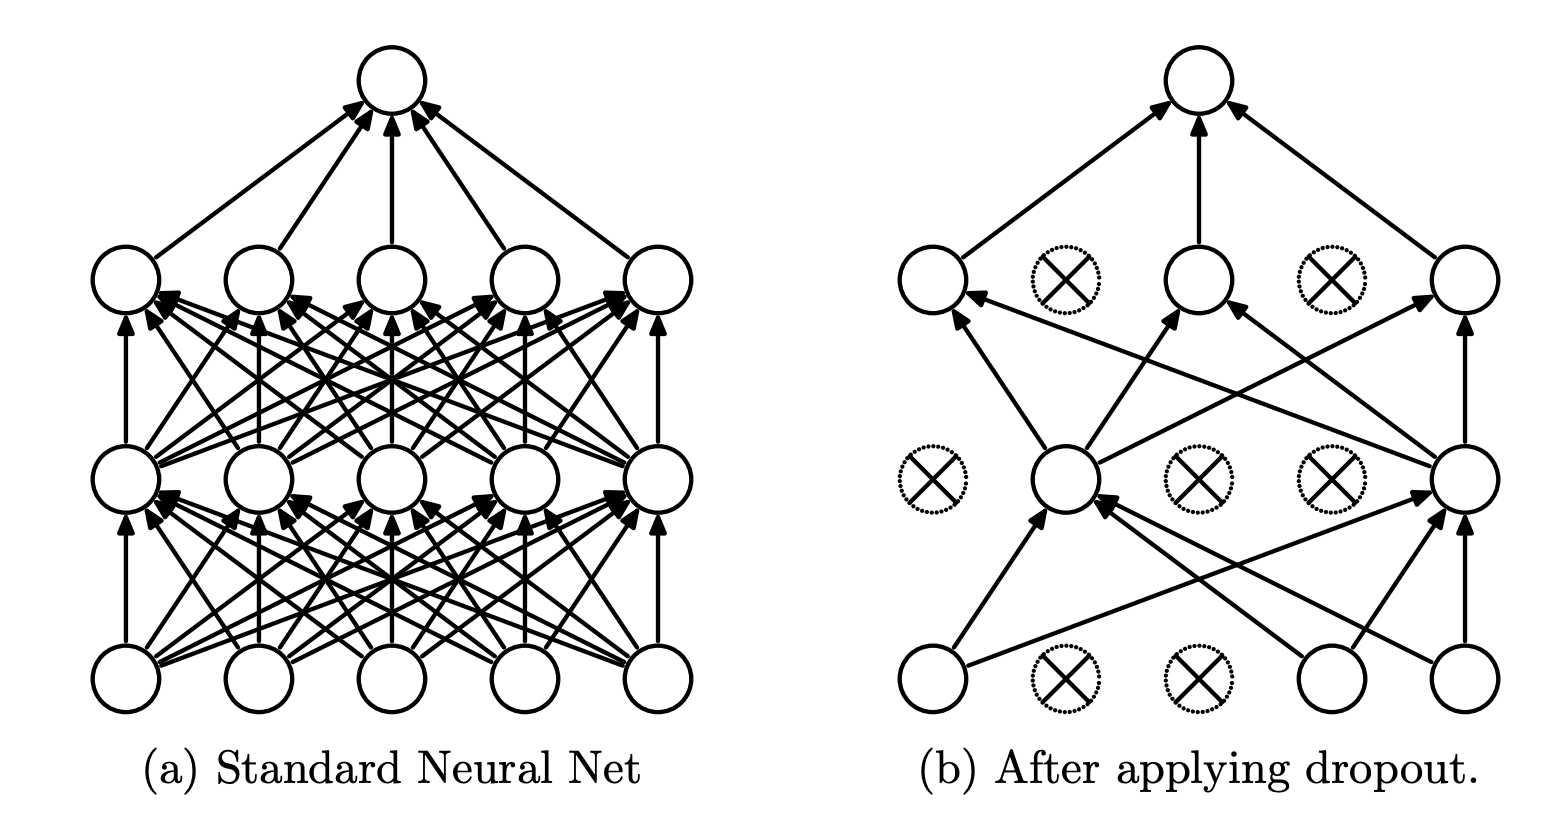
\includegraphics[width=0.5\linewidth]{bilder/dropout.png}
		\caption{Dropout}\label{fig:dropout}
	\end{center}
\end{figure}

\begin{definition}[Activation function]
	An activation function is an element-wise non-linear function $f(\cdot)$. Some examples with are:
	\begin{align}             
		f(x) = \frac{1}{1 + e^{-x}} &&\text{Sigmoid} \\      
		f(x) = max(0, x) &&\text{Rectified linear unit (ReLU)}\\
		f(x) = \begin{cases}
				x, \hspace*{1cm} \textrm{if } x > 0 \\
				\alpha * (e^{x} - 1), \textrm{if }  x \leq 0
		  	\end{cases}\ &&\text{ELU}
		\end{align}
\end{definition}

Models in this work mostly use ELU activations as ELU provides a better signal flow between the layers by not cutting off the negative values completely.

\begin{definition}[UNet]
	UNet is fully convolutional neural network wiht U-shaped encoder-decoder network architecture. [cite Ronneberger].
\end{definition}

The encoder is a usual CNN, consisting of the repeated
block of two $3 \times 3$ convolutions, followed by
an activation function, and a $2 \times 2$ max-pooling operation with stride 2. At each ecnoder step  the number of feature channels doubles. The decoder is also a usual CNN, consisting of repeated blocks of transposed convolution, that halves the
number of feature channels, followed by a concatenation with a corresponding output from an encoder, and two $3 \times 3$ convolutions, followed by a ReLU. The last decoder layer is a $1 \times 1$ convolution to map the tensor to the number of output image channels need. Skip-connections is a very important part of UNet as they allow to the flow of high-resolution features from the encoder to the decoder that in turn allows to restore a corresponding high-resolution image.

\begin{definition}[Autoencoder]
	Autoencoder is an unsupervised learning technique in neural networks for the representation learning purposes. Autoencoder consists of an encoder that compresses data into a lower dimensional representationa and a decoder that restores the original input from the encoded representation.
\end{definition}

\begin{definition}[Overfitting]
    "Hypothesis overfits the training samples if some other hypothesis that fits the training samples less well actually performs better over the entire distribution of instances" (cite p67 Mitchell Machine Learning 1997). They way to avoid overfitting that happened to the models in Sections [TODO cite sections] are discussed in Section [cite regularization section].
\end{definition}
